\documentclass[11pt]{article}

\usepackage{a4wide}
\usepackage{amsmath,amssymb}
\usepackage[english]{babel}
\usepackage{enumitem}
\usepackage{float}
\usepackage{graphicx}
\usepackage[utf8]{inputenc}
\usepackage{listings}
\usepackage{multicol}
\usepackage{tikz}

%========== DEFINITIONS & MACROS ==========%

\definecolor{comment}{rgb}		{0.38, 0.62, 0.38}
\definecolor{keyword}{rgb}		{0.10, 0.10, 0.81}
\definecolor{identifier}{rgb}	{0.00, 0.00, 0.00}
\definecolor{string}{rgb}		{0.50, 0.50, 0.50}

\newcommand{\secref}[1]{see section \ref{#1} on page \pageref{#1}}
\newcommand{\appref}[1]{see appendix \ref{#1} on page \pageref{#1}}
\newcommand{\txtref}[2][]{see {\it #1} \ref{#2} on page \pageref{#2}}
\newcommand{\code}[1]{{\tt #1}}
\newcommand{\file}[1]{{\tt #1}}
\newcommand{\imp}{\rightarrow}
\newcommand{\norm}[1]{\lVert#1\rVert}
\newcommand{\unit}[1]{\frac{#1}{\norm{#1}}}

\setdescription{leftmargin=\parindent, labelindent=\parindent}

\lstset
{
    language=C++,
	% general settings
	numbers=left,
	frame=single,
	basicstyle=\footnotesize\ttfamily,
	tabsize=2,
	breaklines=true,
	% syntax highlighting
	commentstyle=\color{comment},
	keywordstyle=\color{keyword},
	identifierstyle=\color{identifier},
	stringstyle=\color{string},
}


\title
{
    {\Large Individual Assignment 4} \\
    Introduction to Computer Graphics
}

\author
{
    Casper B. Hansen \\
    University of Copenhagen \\
    Department of Computer Science \\
    {\tt fvx507@alumni.ku.dk}
}

\date{last revision \today}

\begin{document}

\clearpage\maketitle\vspace{1in}
\begin{multicols}{2}
    \begin{abstract}
        We will discuss the principles behind light models by taking a look at
        a specific light model; namely, the Phong lighting model.
        
        The reader is not expected to have any prior knowledge of the material
        presented. For the code the reader is expected to have some basic
        understanding of linear algebra and the C++ language.
    \end{abstract}
    \vfill\columnbreak\tableofcontents\vfill
\end{multicols}
\thispagestyle{empty}\newpage

\section{Theory}
A lighting model describes the way in which we interpret how light bounces of
object surfaces in a simulated environment. In this document we will discuss
the Phong lighting model.

The Phong lighting model has three terms; an ambient term ($R_a$) which
describes the minimal amount of emitted reflection bouncing of any surface, a
diffuse term ($R_d$) which describes the surface scattered light bouncing of
surfaces which get hit by a light source, and lastly a specular term ($R_s$)
which describes the light emitted by surface, which in relation to the light
source, reflects light directly at the viewer making the surfaces appear very
bright and shiny.

\begin{figure}[H]
    \begin{align}
        I_p &= \underbrace{k_a l_a}_{R_a}
             + \sum_{l \in \text{lights}}
               \underbrace{k_d l_d (L \cdot N)}_{R_d}
             + \sum_{l \in \text{lights}}
               \underbrace{k_s l_s (R \cdot V)^n}_{R_s}
    \end{align}
    \caption{The Phong lighting model.}
    \label{eqn:phong-light-model}
\end{figure}

The above equation describes the general Phong lighting model with an
arbitrary number of lights in the scene --- hence the summation. The variables
$k$ denote the emissivity of a particular term. That is, {\it how much} a
given term will reflect of the received light. These values are clamped at the
interval $k \in [0;1]$. The variables $l$ denote the light intensities of a
given term.

\subsection{Ambient}
The ambient term of the Phong lighting model is very simple as it omits any
concern of how the surface relates to the light source. By omitting such
detail we regard the light reflection as being equal on any part of a surface.
\begin{figure}[H]
    \begin{align}
        R_a &= k_a l_a
    \end{align}
    \caption{The phong ambient term.}
    \label{eqn:phong-ambient-term}
\end{figure}
Since ambient light is equally distributed among all surfaces we need not
consider how the light hits the surface.

\subsection{Diffuse}
The diffuse term of the Phong lighting model has to take into account how the
light hits the surface.

Consider a surface with normal $N$ getting hit by a light source at position
$l_p$ with intensity $l_i$ from the direction unit vector $L$ and the
direction unit vector $V$ toward the viewer. The light reflected off of the
surface toward the viewer, by Lambert's law, is $k_d l_i \cos \theta = k_d l_i
(L \cdot N)$

\begin{figure}[H]
    \begin{align}
        R_d &= k_d l_d \cos \theta = k_d l_d (L \cdot N)
    \end{align}
    \caption{The phong diffuse term.}
    \label{eqn:phong-diffuse-term}
\end{figure}

If there are multiple lights in the scene, one can extend this by a summation
of the lights as done in the general equation (see
figure~\ref{eqn:phong-light-model})

\subsection{Specular}
The specular term of the Phong lighting model is slightly more involved as
specular highlights are reflected in a small cone around the vector $V$.
Consider such a reflection cone defined by the unit vector $R$ at an angle
$\alpha$ from vector $V$. The emitted light at vector $R$ is the same as that
going in from the light at vector $L$, the angle of which is $\theta$. The
cone $R$ revolving around $V$ can then be expressed as $k_s l_s (R \cdot V)$.
Adding to that the falloff, or {\it shininess}, we can take the $n$th power
of the cosine, which reduces the cone angle $\alpha$, which translates to the
same by putting $R \cdot V$ to the $n$th power.

\begin{figure}[H]
    \begin{align}
        R_s &= k_s l_s \cos^n \alpha = k_s l_s (R \cdot V)^n
    \end{align}
    \caption{The Phong specular term.}
    \label{eqn:phong-specular-term}
\end{figure}

\subsection{Attenuation}
From physics, we can describe a lights falloff rate by the square of the
distance. That is, the attenuation falloff is given by $f_{att} = \frac{1}
{d^2_L}$. We can add this to the general Phong lighting model as shown below.

\begin{figure}[H]
    \begin{align}
        I_p &= \underbrace{k_a l_a}_{R_a}
             + \sum_{l \in \text{lights}}
               f_{att} \underbrace{k_d l_d (L \cdot N)}_{R_d}
             + \sum_{l \in \text{lights}}
               f_{att} \underbrace{k_s l_s (R \cdot V)^n}_{R_s}
    \end{align}
    \caption{The Phong lighting model with attenuation.}
    \label{eqn:phong-attenuation}
\end{figure}

This will effectively make distant objects appear darker than those closer to
a light source, which is a closer approximation of how real object surfaces
reflect light.

\subsection{Surface Colors}
Now that we have a model for which we can describe how much light is reflected
off of a surface, we can turn our attention toward what color the surface
reflects and how to add it to our equation.

A surface reflection coefficients $k$ in conjunction with surface reflection
colors $O$ form the notion {\it surface material}. Adding these to our
equation, we get the following.

\begin{figure}[H]
    \begin{align}
        I_p &= \underbrace{k_a O_a l_a}_{R_a}
             + \sum_{l \in \text{lights}}
               f_{att} \underbrace{k_d O_a l_d (L \cdot N)}_{R_d}
             + \sum_{l \in \text{lights}}
               f_{att} \underbrace{k_s O_s l_s (R \cdot V)^n}_{R_s}
    \end{align}
    \caption{The Phong lighting model with surface colors.}
    \label{eqn:phong-colors}
\end{figure}

\subsection{Remarks}
The equation we've arrived at (\ref{eqn:phong-colors}) can be reduced to form
a more simple expression that is more easily readable. We can pull out
anything not directly affected by the lights, such as coefficients and colors,
etc. Also, we will employ a shorthand for the surface materials. We will
express these by $k_{q,\lambda} = k_q O_q$, meaning the reflectiveness of
surface property $q$, including the coefficient and color.

\begin{figure}[H]
    \begin{align}
        I_p &= \underbrace{k_a O_a l_a}_{R_a}
             + f_{att} \left( k_{d, \lambda}
               \sum_{l \in \text{lights}} l_d (L_l \cdot N)_{R_d}
             + k_{s, \lambda}
               \sum_{l \in \text{lights}} l_s (R_l \cdot V)^n_{R_s}\right)
    \end{align}
    \caption{The Phong lighting model with surface colors.}
    \label{eqn:phong-final}
\end{figure}

Doing so, we get a much nicer equation that is easy to read. We could reduce
it further by having a single sum, but this, I think, crams the equation.

\newpage
\section{Implementation}
The implementation has a few bugs in it. I intended to write a per-fragment
Phong shader, but it seems that the results are not as expected. I wasn't
able to find the error in time for the deadline, but the shader does indeed
produce Phong shading, just not per-fragment, I think --- again, I'm not sure
as to the source of why it looks like it produces per-vertex result.

\subsection{Vertex Shader}
The vertex shader is given the 3 attributes; \code{vtx}, \code{normal} and
\code{tex}, being the vertex, normal and texture coord attributes. The main
program has been altered since the last assignment to support \code{OBJ} file
loading, which can have all those properties, hence they are present in the
shader as well (lines 3--5).

Because of some issues with the shader, I had to split up the premultiplied
model-view-projection matrix into their separate components and send each one
down to the shader (lines 7--9).

On line 11 we have a uniform for the light position, and line 13 is a uniform
for the shininess factor. Lines 15--16 are varying floats that are passed on
to the fragment shader.

\begin{figure}[H]
    \lstinputlisting[lastline=17]
    {../../src/resources/shaders/phong.shader/vertex.glsl}
    \caption{Code excerpt showing the global variables of the vertex shader.}
    \label{code:vertex-shader-globals}
\end{figure}

On lines 20--21 we compute the eye-coordinate space vectors of the vertex and
normal. On line 23 we compute the $L$ vector, and on the following line 24 we
compute $L_l \cdot N$. On line 26 we compute the $R$ vector, using a helper
function from GLSL, and the $V$ vector on line 27. Then on line 28 $R_l \cdot
V$ is computed, and the specularity is computed on line 29.

Lastly, the position of the vertex in screen space is computed on line 31.

\begin{figure}[H]
    \lstinputlisting[firstnumber=18,firstline=18]
    {../../src/resources/shaders/phong.shader/vertex.glsl}
    \caption{Code excerpt showing the vertex shader progam.}
    \label{code:vertex-shader}
\end{figure}

\subsection{Fragment Shader}
In the fragment shader, since most of the work has been hoisted up the
pipeline ---improving the efficiency---, lines 3--14 are merely the uniforms
we send to the shader, and lines 16--17 are the varying floats we passed from
the vertex shader.

\begin{figure}[H]
    \lstinputlisting{../../src/resources/shaders/phong.shader/fragment.glsl}
    \caption{Code excerpt showing the fragment shader.}
    \label{code:fragment-shader}
\end{figure}

The $R_a$, $R_d$ and $R_s$ are calculated on lines 21--23, and summed on line
25.

\subsection{Tests}
The program source code allows for moving and rotating a teapot object, which
is being loaded from an \code{OBJ}-file. This should allow for easy
verification of the test screenshots provided below.

\begin{figure}[H]
    \center
    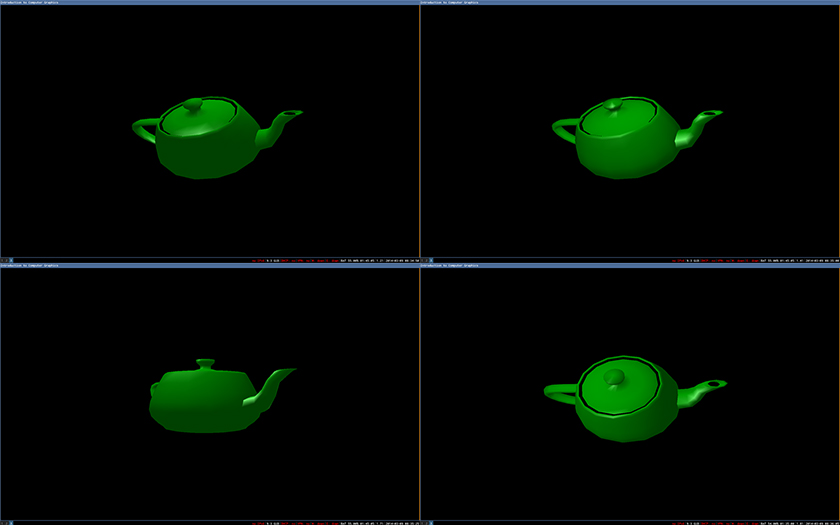
\includegraphics[scale=0.5]{figures/screenshots}
    \caption{Screenshots showing the Phong shader on a teapot.}
    \label{code:test-screenshots}
\end{figure}

\end{document}

